\subsection{Caso peggiore metodo divisione} \label{caso_peggiore_div}
Seguendo la filosofia \textit{worst case analysis}, osserviamo il comportamento della tabella quando sono assegnati i valori critici per il metodo della divisione. \\
Impostiamo quindi: $m = 2^{p}$ (in questo caso $m = 16$) e tutte le chiavi $k$ degli utenti \verb|User| tra loro multiple di $m$, ovvero ad esempio $16,32,48,64$ etc.
Inseriamo in tutto $11$ oggetti in tabella così da avere alla fine come \textit{load factor} $\alpha = n/m \approx 70\%$.

Possiamo eseguire il tutto con il seguente \textit{snippet} di codice che invocherà i metodi implementati:

% multiline code snippet
\lstset{
      basicstyle=\small,
      xleftmargin=.1\textwidth,
}
\begin{lstlisting}
key = m
for i in range(11):
    Hash.insert(User(key, string.ascii_uppercase[i]))
    key + = m
\end{lstlisting}


In questo modo tutti gli oggetti hanno come chiave \verb|key| un multiplo di $m$ e come attributo \verb|value| una lettera dell'alfabeto (da \verb|"a"| fino a \verb|"k"| essendoci in tutto $11$ elementi).

\begin{figure}[htb]
    \begin{center}
    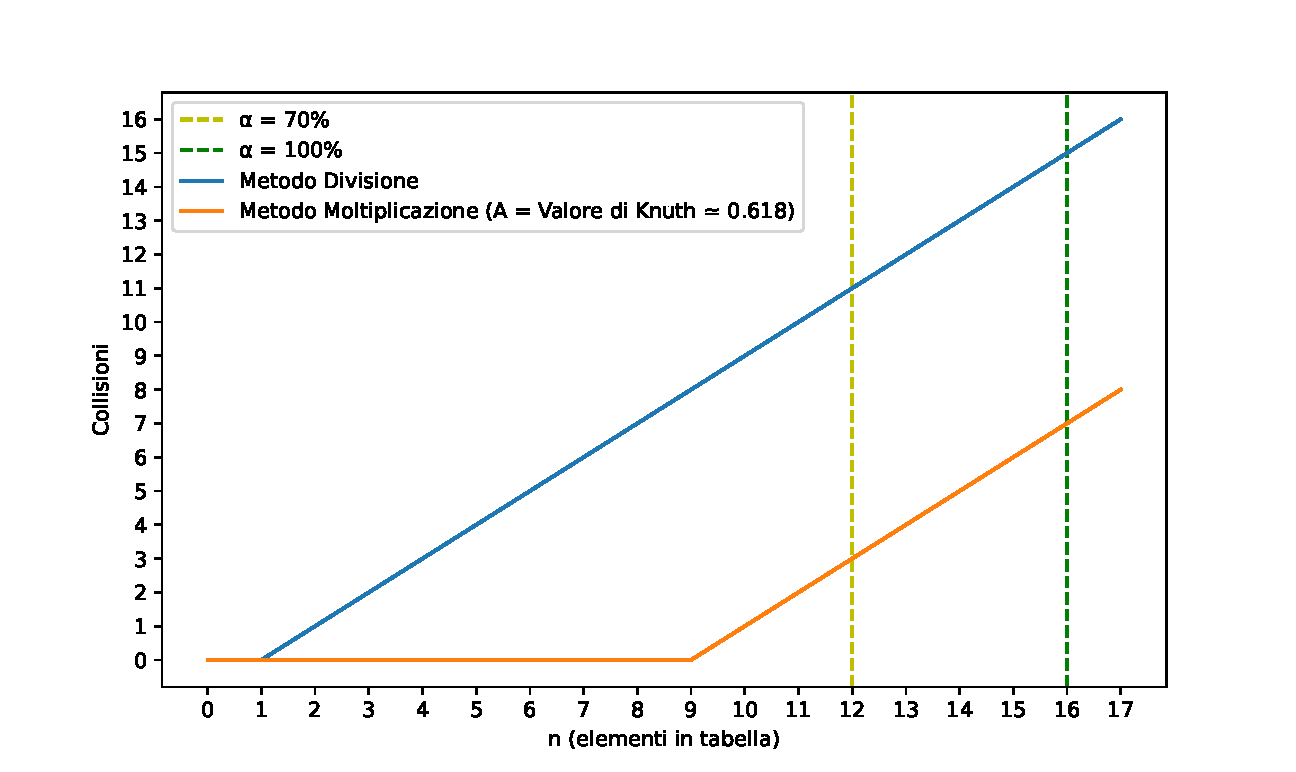
\includegraphics[scale=0.65]{src/img/worstcase.pdf}
    \caption{Caso peggiore metodo della divisione}
     \label{fig:met_div}
    \end{center}
\end{figure}

Come si nota in Figura \ref{fig:met_div}, il metodo della divisione risulta pessimo: dopo il primo elemento inserito, abbiamo tutte e sole collisioni.
\\ Viceversa il metodo della moltiplicazione grazie alla sua funzione di hash apparentemente casuale riesce a gestire assai meglio la situazione, e si rilevano due sole collisioni rispettivamente quando si inserisce il decimo e l'undicesimo elemento. In Figura \ref{fig:tikz:worstcase} è riportata la struttura grafica della tabella.

\begin{figure}[htp]
  Tabella T1 (metodo divisione):

\begin{tikzpicture}
\coordinate (0);
\foreach \t/\n[count=\i from 0,evaluate=\i as\j using int(\i+1)] in {
 K $\rightarrow$ J $\rightarrow$ I $\rightarrow$ H $\rightarrow$ G $\rightarrow$ F $\rightarrow$ E $\rightarrow$ D $\rightarrow$ C $\rightarrow$ B $\rightarrow$ A/ ,
 ,
 ,
 ,
 ,
 ,
 ,
 ,
 ,
 ,
 ,
 ,
 ,
 ,
 ,
}
\node at(\i.south)[anchor=north,draw,minimum height=1.4em,minimum width=2.5em,outer sep=0pt](\j){\n}
    node at(\j.west)[align=right,left]{\i} 
    node at(\j.east)[align=left,right,xshift=-.7em]{$\rightarrow$ \t};
\end{tikzpicture}

\vspace{20pt}
Tabella T2 (metodo moltiplicazione):

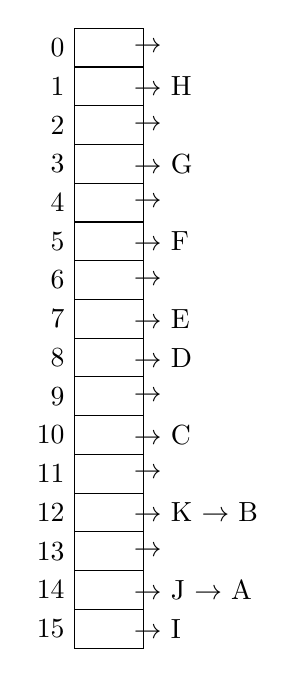
\begin{tikzpicture}
\coordinate (0);
\foreach \t/\n[count=\i from 0,evaluate=\i as\j using int(\i+1)] in {
 ,
 H/,
 ,
 G/,
 ,
 F/,
 ,
 E/,
 D/,
 ,
 C/,
 ,
 K $\rightarrow$ B/,
 ,
 J $\rightarrow$ A/,
 I/
}
\node at(\i.south)[anchor=north,draw,minimum height=1.4em,minimum width=2.5em,outer sep=0pt](\j){\n}
    node at(\j.west)[align=right,left]{\i} 
    node at(\j.east)[align=left,right,xshift=-.7em]{$\rightarrow$ \t};
\end{tikzpicture}

\newpage
  \caption{Le due tabelle del caso \ref{caso_peggiore_div} a confronto.}
  \label{fig:tikz:worstcase}
\end{figure}

\textit{Nota}: l'andamento delle collisioni con il metodo della moltiplicazione cresce in modo lineare (quindi critico) dopo che il \textit{load factor} supera i valori massimi di riferimento. Motivo per il quale in questi casi è consigliato ridimensionare la tabella, ad esempio raddoppiando il valore di \textit{m}.
